\documentclass[conference]{IEEEtran}
\usepackage{mathptmx} % Times New Roman font
\usepackage{graphicx}
\usepackage{array}
\usepackage{cite}
\usepackage{amsmath}
\usepackage{balance} % For balancing last page columns
\usepackage{tikz}
\usetikzlibrary{arrows.meta, positioning}
\usepackage{graphicx} % Required for images

% Set margins for US Letter paper
\usepackage[letterpaper,
            left=0.625in,
            right=0.625in,
            top=0.75in,
            bottom=1in]{geometry}

% Section numbering with Roman numerals
\renewcommand{\thesection}{\Roman{section}}
\renewcommand{\thesubsection}{\Alph{subsection}}

\begin{document}

\title{Implementation and In-Depth Analysis of Flight Optimization Systems for Travel Agencies: A Multi-Criteria Approach}

\author{Yasin Yeşilyurt\\
TOBB ETÜ Artificial Intelligence
Engineering\\
Söğütözü cad. TOBB ETÜ Konukevi\\
Yenimahalle/Ankara\\
yasinyesilyurt@hotmail.com}

\maketitle

\begin{abstract}
This paper presents a multi-criteria flight optimization system for travel agencies, designed to recommend optimal flight routes by balancing cost, duration, and customer satisfaction. 
The proposed framework employs A*, Dijkstra's, and Genetic Algorithms implemented in Python to evaluate flight data spanning 1993-2023 from U.S. domestic routes, sourced from a Kaggle dataset containing 245,955 entries with parameters such as fare, distance, carrier dominance, and airport coordinates. 
Key innovations include a hybrid approach combining heuristic pathfinding (using Haversine distance for A*) with multi-objective A* to address multi-objective optimization. 
Results demonstrate the effectiveness of A* and Dijkstra's algorithms in minimizing travel costs and time, while genetic algorithm gives sufficient results, it is much slower than mentioned algorithms without proper optimization techniques. 
The system currently provides personalized flight recommendations based on user preferences, with visualized outputs generated via the NetworkX library.
This work contributes a scalable framework for enhancing decision-making in travel planning systems.
\end{abstract}

\section{INTRODUCTION}
The growing complexity of air travel planning necessitates advanced systems to optimize flight routes while balancing competing factors such as cost, duration, and customer satisfaction. 
Traditional travel recommendation tools often prioritize single objectives, such as minimizing price or travel time, but fail to account for multi-dimensional preferences or dynamic market conditions. 
This limitation underscores the need for intelligent systems capable of synthesizing diverse parameters to deliver personalized and context-aware solutions.\\

Existing approaches to route optimization predominantly rely on classical graph algorithms like Dijkstra's or heuristic methods such as A*. 
However, these methods struggle to handle multi-criteria optimization, where trade-offs between conflicting objectives (e.g., cost vs. comfort) must be quantified. 
While recent studies have explored hybrid frameworks combining machine learning and optimization techniques, their reliance on simplified datasets or synthetic benchmarks limits real-world applicability.\\

This paper addresses these gaps by proposing a hybrid algorithmic framework that integrates A* (heuristic Search), Dijkstra's algorithm (shortest-path), and Genetic Algorithms (evolutionary optimization) to optimize flight routes across three criteria: fare, travel time, and carrier-specific customer satisfaction metrics. 
The system leverages a comprehensive dataset of 245,955 U.S. domestic flights (1993-2023), which includes real-world attributes such as historical fares, carrier dominance, and geographic coordinates. 
Key innovations include:
\begin{itemize}
    \item A Haversine-based heuristic for A* to compute geodesic distances between airports, improving route accuracy.
    \item A genetic crossover mechanism to evolve flight paths while preserving high-quality route segments.
    \item A dynamic weighting system to prioritize user-defined preferences (e.g., cost-sensitive vs. time-sensitive travelers).
    \item A multi-objective A* algorithm that evaluates trade-offs between fare, travel time, and customer satisfaction, enabling personalized recommendations.
    \item Visualization of flight networks and optimized routes using the NetworkX library, enhancing decision-making.
\end{itemize}
Preliminary results demonstrate the viability of A* and Dijkstra's algorithms for single-objective optimization but the genetic algorithm exhibits slower performance. 
Among the mentioned algorithms A* performs best in terms of cost and time minimization thus it has been selected as multi-criteria optimizer. 
The remainder of this paper is organized as follows: Section II details the methodology and dataset, Section III discusses implementation challenges and results, and Section IV outlines future work to refine hybrid algorithm performance and integrate real-time customer feedback.


\section{METHODOLOGY}
The proposed flight optimization system follows a structured pipeline (Fig. 1) comprising data preprocessing, algorithmic implementation, and multi-criteria evaluation.  
\subsection{Data Collection and Preprocessing}
A dataset of 305,189 U.S. domestic flights (1993–2023) [1] was sourced from Kaggle, containing attributes such as fares, carriers, passenger counts, airport coordinates, and quarterly trends. Key preprocessing steps include:  
\begin{itemize}
    \item 1. Data Cleaning: Removal of 105,189 incomplete entries, retaining 200,000 flights with non-null values.  
    \item 2. Subset Selection: Partitioning by year and quarter to reduce computational load.  
    \item 3. Graph Construction: Representing airports as nodes and flights as edges in a weighted graph using Python’s `NetworkX` library. Edge weights combine:  
    \begin{description}
        \item [Cost] Normalized fare (\$) scaled by carrier dominance (market share).  
        \item [Time] Flight duration derived from Haversine distance (km) between coordinates.  
    \end{description}   

\end{itemize}

Workflow diagram of the flight path finder pipeline is shown in Fig. \ref{fig:pipeline}.
\begin{figure}[htbp]
    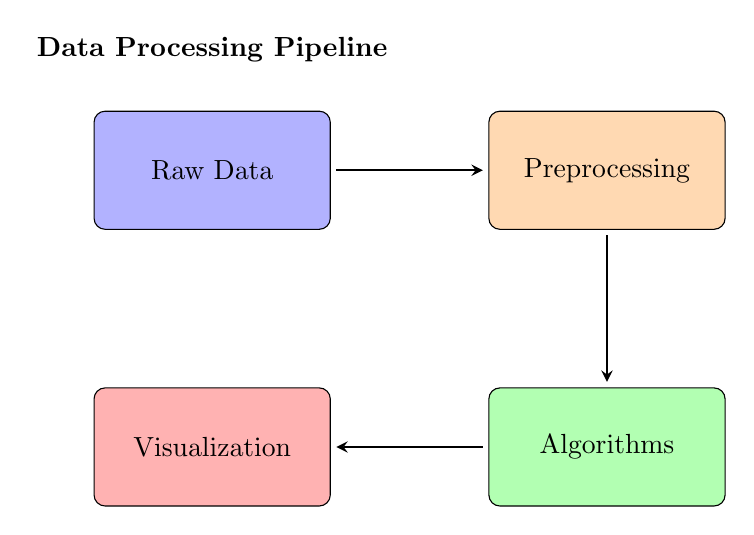
\begin{tikzpicture}[
        node distance=2cm,
        stage/.style={
            rectangle, 
            rounded corners, 
            minimum width=3cm, 
            minimum height=1.5cm, 
            text centered, 
            draw=black, 
            fill=blue!30
        },
        arrow/.style={
            thick, 
            -stealth, 
            shorten >=2pt, 
            shorten <=2pt
        }
    ]
    
    % Nodes
    \node (data) [stage, fill=blue!30] {Raw Data};
    \node (preprocessing) [stage, fill=orange!30, right=of data] {Preprocessing};
    \node (algorithms) [stage, fill=green!30, below=of preprocessing] {Algorithms};
    \node (visualization) [stage, fill=red!30, left=of algorithms] {Visualization};
    
    % Arrows
    \draw [arrow] (data) -- (preprocessing);
    \draw [arrow] (preprocessing) -- (algorithms);
    \draw [arrow] (algorithms) -- (visualization);
    
    % Title
    \node[above=0.5cm of data, font=\bfseries] {Data Processing Pipeline};
    
    \end{tikzpicture}
    \caption{Flight path finder pipeline workflow from data to visualization}
    \label{fig:pipeline}
\end{figure}

\subsection{Algorithm Design} 
Three core algorithms with a multi-objective variant of these algorithms were implemented and compared:  

\begin{enumerate}
    \item A* Algorithm:  
        \begin{itemize}
            \item Heuristic Function: Geodesic distance between airports computed via the Haversine formula:  
              \[
              d = 2R \arcsin\sqrt{\sin^2\left(\frac{\Delta\phi}{2}\right) + \cos\phi_1 \cos\phi_2 \sin^2\left(\frac{\Delta\lambda}{2}\right)}
              \]  
              where \(R\) is Earth's radius, and \(\phi\), \(\lambda\) denote latitude/longitude.  
            \item Cost Function: \(C = \alpha \cdot \text{fare} + \beta \cdot \text{distance}\).  
        \end{itemize}
    
    \item Dijkstra's Algorithm:  
        \begin{itemize}
            \item Computes globally optimal paths for a single criterion (e.g., minimal distance).  
            \item Extended to support dynamic reweighting of edges based on user preferences.  
        \end{itemize}
    
    \item Genetic Algorithm (GA):  
        \begin{itemize}
            \item Population Initialization: 100 chromosomes generated via greedy random walks.  
            \item Crossover: Segments of parent paths sharing common nodes (e.g., P1: A→B→C→D and P2: A→X→C→Y yield children A→B→C→Y and A→X→C→D).  
            \item Mutation: Random node insertion/deletion (currently disabled due to instability in variable-length paths).  
            \item Fitness Function: Minimizes \(cost\) while penalizing excessive layovers.  
        \end{itemize}
    \item Multi-Criteria A* Algorithm:  
        \begin{itemize}
            \item Heuristic Function: Haversine distance as in A*.
            \item Cost Function: follows in Fig \ref{fig:my_image}.
            \item Cost Function: \(C = \alpha \cdot \text{fare} + \beta \cdot \text{distance}\). 
        \end{itemize}
\end{enumerate}

\begin{figure}[htbp]
    \centering
    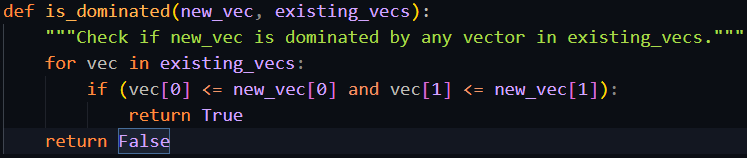
\includegraphics[width=0.486\textwidth]{domination.png} % Replace with your filename
    \caption{Pareto Optimal checker for Multi-Criteria A* Algorithm}
    \label{fig:my_image}
\end{figure}


\section{Implementation Details}
\begin {itemize}
    \item Environment: Python 3.9, Jupyter Notebook for interactive development.  
    \item Libraries: `NetworkX` for graph representation, `pandas` for data manipulation, `numpy` for numerical operations.  
    \item Visualization: Matplotlib and NetworkX for geographic rendering of flight paths.
\end{itemize}  


\subsection{Challenges and Mitigations}

\subsubsection{Data Completeness and Geographic Accuracy}
\begin{itemize}
    \item Challenge: Initial datasets lacked geographic coordinates for airport entries, compromising distance calculations.
    \item Mitigation: Found a different dataset that included most of its airport coordinates.
\end{itemize}

\subsubsection{Computational Bottlenecks}
\begin{itemize}
    \item Challenge: Rendering 200,000+ flights in \texttt{NetworkX} caused latency. 
    \item Mitigation: Visualization was limited to 50--100 nodes when testing, complete graphs are rendered afterwards.
\end{itemize}

\subsubsection{Multi-Parameter Optimization}
\begin{itemize}
    \item Challenge: No standard function to unify cost, time, and comfort metrics. 
    \item Mitigation: A user-configurable weighted sum (e.g., 20\% cost, 80\% distance) and multi-parameter A* was implemented. 
\end{itemize}

\subsubsection{Genetic Algorithm Implementation}
\begin{itemize}
    \item Challenge 1: Python's list/tuple structures caused inefficient chromosome representation. That caused shape mismatch errors during crossover and mutation operations.
    \item Mitigation: Mutation instability was resolved by enforcing path continuity checks during chromosome editing. But a more planned chromosome representation is recommended for future work.
    
    \item Challenge 2: Random Heuristic Walk algorithm caused mutations to be mostly longer paths. This caused mutated chromosomes to be longer than the original ones. 
    \item Mitigation: Implemented a natural selection (sorting the chromosomes by their length) is implemented.
\end{itemize}

% \begin{table}[ht]
% \centering
% \caption{Type Sizes for Papers}
% \label{tab:type}
% \begin{tabular}{|l|l|l|l|}
% \hline
% \textbf{Type size (pts.)} & \textbf{Regular} & \textbf{Bold} & \textbf{Italic} \\ \hline
% 6 & Table captions & & \\ \hline
% 8 & Section titles & & \\ \hline
% 9 & Main text & Abstract & Subheading \\ \hline
% 10 & Authors' names & & \\ \hline
% 11 & Paper title & & \\ \hline
% \end{tabular}
% \end{table}

% \section{HELPFUL HINTS}
% \subsection{Figures and Tables}
% Position figures and tables at the tops and bottoms of columns. Figure captions should be centered below the figures as shown in Fig.~\ref{fig:sample}.

% \begin{figure}[ht]
% \centering
% % \includegraphics[width=3in]{sample-figure}
% \caption{Sample figure caption.}
% \label{fig:sample}
% \end{figure}

% \subsection{References}
% Number citations consecutively in square brackets~\cite{ref1}. Use ``Ref.~[3]'' at the beginning of a sentence. 

% \subsection{Equations}
% Number equations consecutively:
% \begin{equation}
% a + b = c
% \end{equation}
% Symbols should be defined immediately following the equation.

% \section{UNITS}
% Use either SI (MKS) or CGS as primary units. Avoid combining SI and CGS units.

% \section{SOME COMMON MISTAKES}
% The word ``data'' is plural. Use proper punctuation within quotation marks: ``like this.'' 

% \section*{ACKNOWLEDGMENT}
% The preferred spelling is ``acknowledgment'' without an ``e'' after the ``g.''

\balance % Balance columns on last page

\begin{thebibliography}{9}
\bibitem{ref1} G. Eason et al., ``On certain integrals,'' Phil. Trans. Roy. Soc. London, vol. A247, pp. 529-551, 1955.
\bibitem{ref2} J. Clerk Maxwell, A Treatise on Electricity and Magnetism. Oxford: Clarendon, 1892.
\end{thebibliography}

\end{document}